\documentclass[a4paper,11pt]{article}
\usepackage{commonpackages}

\begin{document}
\title{Trigonométrie dans le triangle rectangle}
\date{}
\maketitle

\section{Théorie}
\subsection{Définition}
\begin{multicols}{2}
Soit le triangle rectangle $ABC$ rectangle en $C$. Par rapport à l'angle $\alpha$, $a$ est le \textbf{côté opposé}, $b$ est le \textbf{côté adjacent} et $c$ est l'\textbf{hypoténuse}.\\
\begin{center}
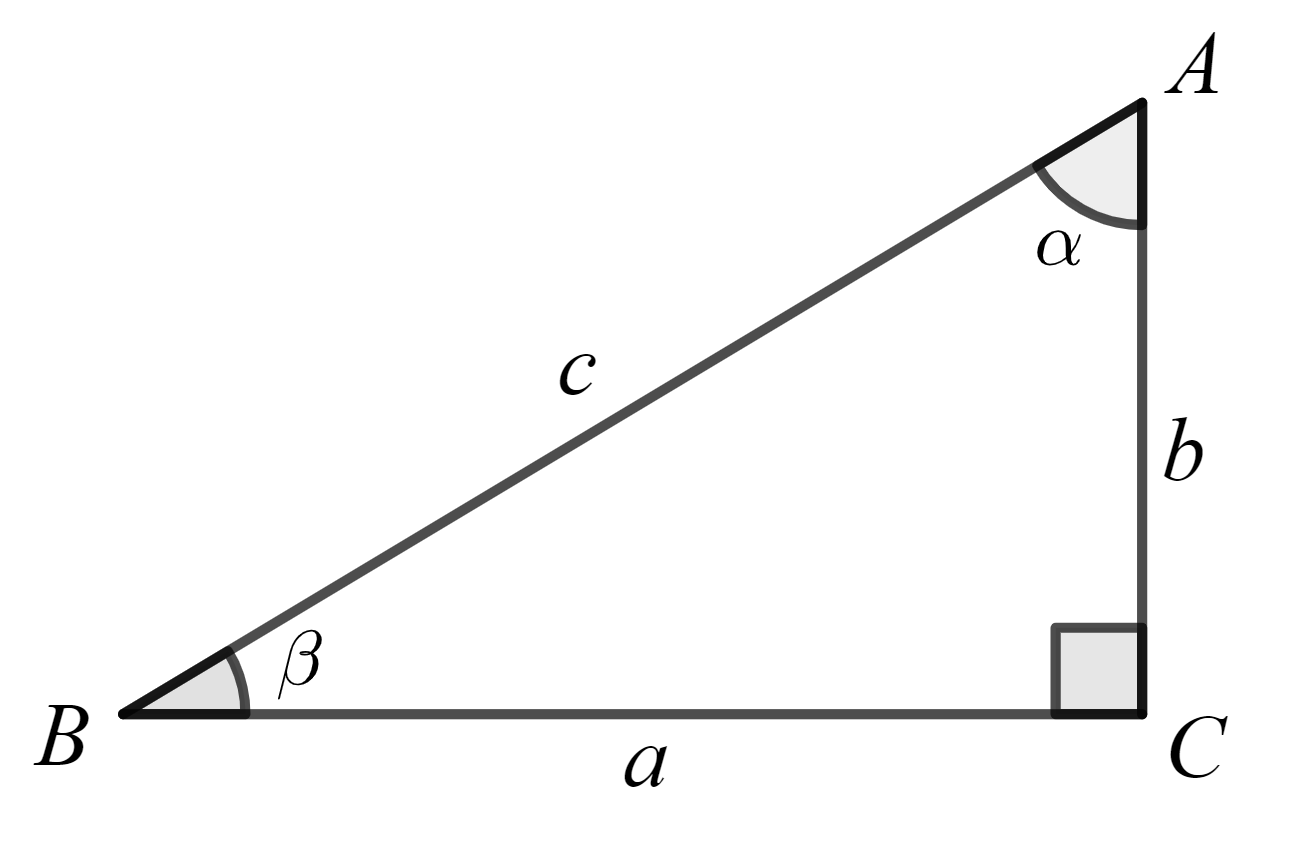
\includegraphics[width=0.8\textwidth]{images/trianglerect.png}\\
\end{center}
\end{multicols}

\subsection{Théorème}
Soit $\alpha$ un des deux angles aigus d'un triangle rectangle. Le rapport du côté opposé de $\alpha$ et de l'hypoténuse est appelé \textbf{sinus de $\alpha$} et nous écrivons
$$\sin(\alpha)=\frac{\text{opposé de }\alpha}{\text{hypoténuse}}$$

Le rapport du côté adjacent de $\alpha$ et de l'hypoténuse est appelé \textbf{cosinus de $\alpha$} et nous écrivons

$$\cos(\alpha)=\frac{\text{adjacent de }\alpha}{\text{hypoténuse}}$$

Le rapport du côté opposé de $\alpha$ et du côté adjacent de $\alpha$ est appelé \textbf{tangente de $\alpha$} et nous écrivons

$$\tan(\alpha)=\frac{\text{opposé de }\alpha}{\text{adjacent de }\alpha}$$


\section{Exemple}
Dans un triangle rectangle en $C$, nous connaissons $\alpha=27^{\circ}$ et $c=8\,cm$. Résoudre ce triangle.\\
\begin{multicols}{2}
\begin{center}
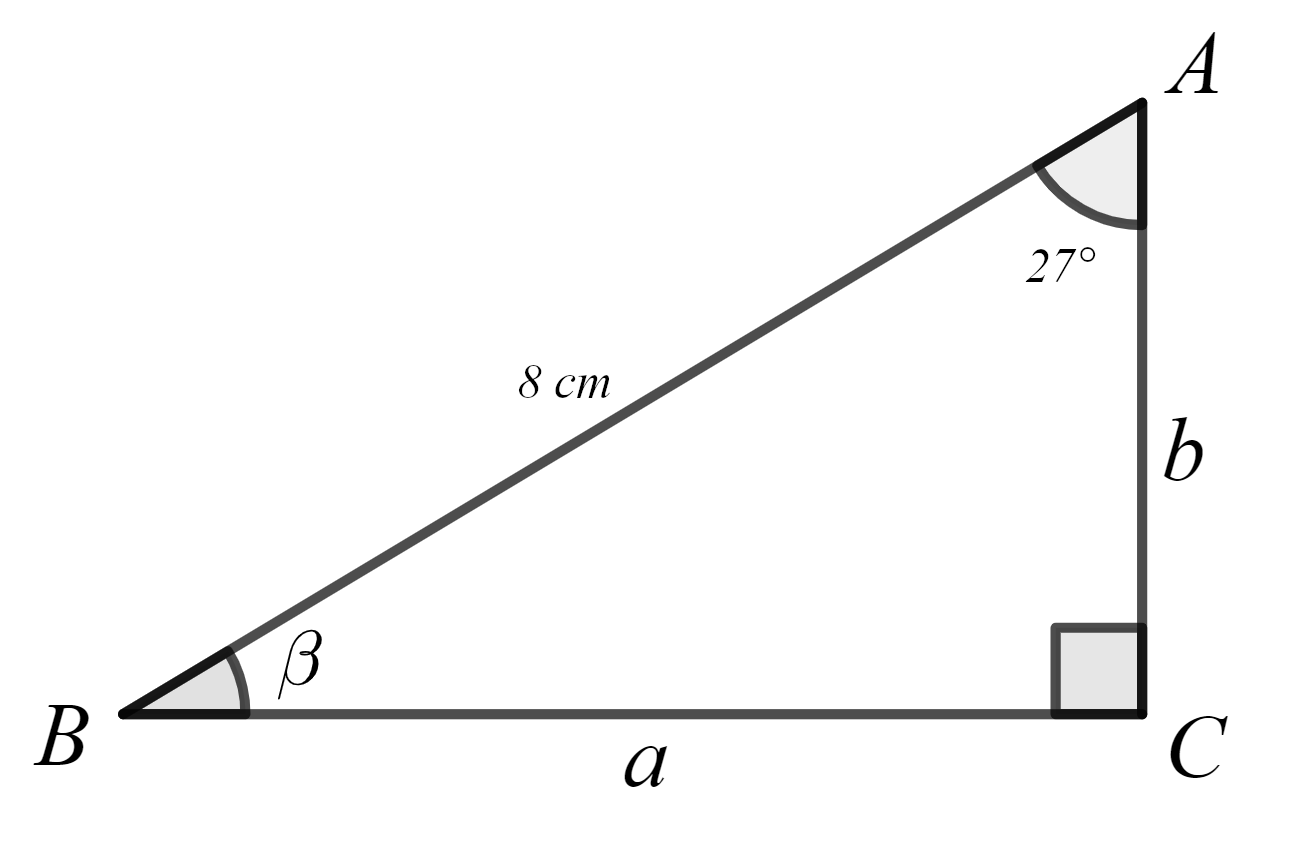
\includegraphics[width=0.8\textwidth]{images/trianglerectexemple.png}\\
\end{center}
$\beta=180-90-27=63°$\\
En utilisant la trigonométrie:\\
$\sin(\alpha)=\dfrac{\text{opp}}{\text{hyp}} \Rightarrow \sin(27)=\dfrac{\overline{BC}}{8}$\\
$\Rightarrow \overline{BC}=8 \cdot \sin(27)=3.63\,cm$\\
$\cos(\alpha)=\dfrac{\text{adj}}{\text{hyp}} \Rightarrow \cos(27)=\dfrac{\overline{AC}}{8}$\\
$\Rightarrow \overline{AC}=8 \cdot \cos(27)=7.13\,cm$\\
\end{multicols}

\section{Vidéos}
Théorie et exemple\\
\video{DfgUYXB5_jg} \video{BscM5Iti3zI}


\section{Exercice}
Dans le tableau ci-dessous, il s'agit de triangle rectangle en $C$. Compléter le tableau.
\begin{center}
\begin{tabular}{ | c | c | c | c | c | }
  \hline
 $\phantom{texte}\alpha\phantom{texte}$ & $\phantom{texte}\beta\phantom{texte}$ \phantom{texte}& $\phantom{texte}a\phantom{texte}$ & $\phantom{texte}b\phantom{texte}$ & $\phantom{texte}c\phantom{texte}$   \\
   \hline
 $35^{\circ}$ &  & $10$ &  &    \\
   \hline
  & $10^{\circ}$ & $15$ &  &    \\
   \hline
$70^{\circ}$  &  &  &  &  $8$  \\
   \hline
  &  & $3$ & $4$  &    \\
   \hline
  & $100^{\circ}$ &  & $5$ &    \\
   \hline
  &  & $8$ &  &  $10$  \\
   \hline
\end{tabular}
\end{center}

\begin{solution}
\begin{center}
\begin{tabular}{ | c | c | c | c | c | }
  \hline
 $\phantom{texte}\alpha\phantom{texte}$ & $\phantom{texte}\beta\phantom{texte}$ \phantom{texte}& $\phantom{texte}a\phantom{texte}$ & $\phantom{texte}b\phantom{texte}$ & $\phantom{texte}c\phantom{texte}$   \\
   \hline
 $35^{\circ}$ & $55^{\circ}$ & $10$ & $14.28$ & $17.43$   \\
   \hline
 $80^{\circ}$ & $10^{\circ}$ & $15$ & $2.64$ & $15.23$   \\
   \hline
$70^{\circ}$  & $20^{\circ}$ & $7.52$ & $2.74$ &  $8$  \\
   \hline
$36.87^{\circ}$  & $53.13^{\circ}$ & $3$ & $4$  & $5$   \\
   \hline
 Pas & $100^{\circ}$ & pos- & $5$ &  sible  \\
   \hline
 $53.13^{\circ}$ & $36.87^{\circ}$ & $8$ & $6$ &  $10$  \\
   \hline
\end{tabular}
\end{center}
\end{solution}

\section{Plus d'exercices}
\href{https://www.gomaths.ch/print_trigo.php?find=3&nb_calcul=10}{gomath}

\end{document}
